\section{Methodology}\label{sec:methodology}
This section details the mathematical framework developed to quantify the demand-side flexibility of a data centre by co-optimising its primary subsystems. The conceptual model of the data centre, illustrated in Figure~\ref{fig:dc_layout}, integrates three dynamically coupled components: the IT systems, which process both flexible and inflexible computational workloads; the power infrastructure, featuring an Uninterruptible Power Supply which operates as an Energy Storage System (UPS-ESS); and the cooling infrastructure, which includes a chiller coupled with a Thermal Energy Storage (TES) tank and the CRAC system. 

Our approach is centred on a comprehensive optimisation model that captures the operational dynamics and physical constraints of each subsystem. Flexibility is harnessed from three key sources: (1) shifting  IT workloads in time, (2) strategically charging and discharging the UPS-ESS, and (3) strategically managing the cooling system by utilising the TES and the inherent thermal inertia of the facility. By integrating these components into a unified framework, the data centre's total capacity to modulate its electricity consumption is evaluated, thereby quantifying its potential to provide valuable grid services.

\rev{The model is intentionally aggregate rather than a server-level or device-level digital twin. The objective of this work is to quantify the flexibility potential available to the power system from a data centre, not to reproduce the detailed operational behaviour of individual servers or cooling devices \cite{barroso2018datacenter,dayarathna2015data}. The modelling therefore prioritises the state variables that determine flexibility feasibility: CPU utilisation and delay tolerance for IT work, UPS state of charge and converter limits for electrical storage, TES state of charge and facility temperatures for cooling recovery, and total grid power for service delivery. Likewise, the purpose of the cooling model is to capture the energy-flexibility interaction between thermal storage, cooling demand and electricity consumption, rather than detailed airflow dynamics within server racks. This abstraction preserves the operational couplings that matter for flexibility while keeping the repeated optimisation solves required by the flexibility assessment computationally tractable. Importantly, the required computational work of every IT job is always executed in full within its delay tolerance, so flexibility is provided without sacrificing computational throughput or service quality.}


The revised implementation applies this integrated model across the complete
2025 calendar year. Rather than solving 365 independent days, it links the
physical state and unfinished computational work from one local day to the next.
Each local-day optimisation contains a committed core and a three-hour look
ahead, and the detailed annual handoff procedure is given at the end of this
section. The component models are first presented in the same order as the
original formulation so that the role and revision of each equation remain
transparent.

\subsection{IT Workload Methodology}
 
In the literature, there is no consensus on IT workload characteristics and utilisation levels, as they vary significantly depending on the data centre size, type (e.g., enterprise, colocation, hyperscale) and workload nature (e.g., banking, AI). Consequently, even publicly available real-world datasets can differ substantially across facilities. Chris Zaloumis \cite{Zaloumis2022IBM} indicates that average CPU utilisations vary between 12\% and 18\% of total capacity, while Ankur Ghia's findings indicate a daily average between 20\% and 30\%, noting that best practices can elevate this to 70\%--80\% \cite{Ghia2011McKinsey}. 
 
 A study by Google \cite{6779441} classified data centre workloads into four categories based on their sensitivity to delay, labelled from ``0'' (least sensitive) to ``3'' (most sensitive). If categories 2 and 3 are considered inflexible, they account for approximately 30\% of the total workloads, suggesting that up to 70\% of the workloads could be flexible. Another study by Cao et al. \cite{Cao2022ApEn}, conducted using Alibaba's cluster trace, found that inflexible workloads represent 60\% of all jobs but contribute only 30\% of total energy consumption. In contrast, flexible workloads constitute 40\% of jobs while consuming 70\% of the energy. Furthermore, studies such as \cite{Misaghian2023TIA,Xu2023SPIE,Zhou2024IJEPES,Fu2020ApEn,Liu2012PER} reveal that there is no universally accepted ratio, and the estimated shares of flexible and inflexible IT workloads differ significantly across studies for a typical 24-hour period. 

Based on the review of the literature, a dataset of reported workload ratios and graphs over a 24-hour time horizon was compiled. From this dataset, the minimum and maximum values were extracted, and the average ratio was computed, separately for flexible, inflexible, and total workloads relative to total CPU capacity. Drawing upon these values, the workload ratio assumptions adopted in this study were established and are presented under the ``Proposed'' category in Table~\ref{tab:workload-rates}. \rev{The evidence base used to construct these assumptions is consolidated in Table~\ref{tab:workload-source-summary}. Reported hourly workload ratios and graphical profiles were tabulated or digitised where required and grouped into flexible, inflexible and total workload categories. For each hour, the minimum, maximum and average reported values were computed, and the proposed value was selected as a representative profile within the observed range while preserving the daily shape and the aggregate balance between flexible and inflexible demand. The ``Proposed'' columns therefore constitute modelling assumptions synthesised from the literature rather than measurements from a single facility.}

\begin{table}[!t]
\centering
\caption{\rev{Evidence Used to Construct the Workload Assumptions}}
\label{tab:workload-source-summary}
\begin{scriptsize}
\rev{%
\begin{tabular}{p{0.22\columnwidth}p{0.28\columnwidth}p{0.35\columnwidth}}
\toprule
\textbf{Evidence type} & \textbf{Sources} & \textbf{Use in this study} \\
\midrule
Observed utilisation ranges & \cite{Zaloumis2022IBM,Ghia2011McKinsey} & Bounds and representative average CPU utilisation levels. \\
Delay-sensitivity classes & \cite{6779441} & Mapping of workload classes into flexible and inflexible groups. \\
Batch-workload flexibility & \cite{Cao2022ApEn} & Flexible/inflexible workload energy shares and periodic workload shifting behaviour. \\
Flexibility case studies & \cite{Misaghian2023TIA,Xu2023SPIE,Zhou2024IJEPES,Fu2020ApEn,Liu2012PER} & Cross-checking plausible daily workload shapes and flexibility ranges. \\
\bottomrule
\end{tabular}}%
\end{scriptsize}
\end{table}


% --- Single-column version (keeps original formatting) ---
\begin{table}[!t]
\centering
\caption{IT Workload Rates}\label{tab:workload-rates}
\begin{scriptsize}
\setlength{\tabcolsep}{3pt}
\resizebox{\columnwidth}{!}{%
\begin{tabular}{lrrrrrrrrrrrrr}
\toprule
{\textbf{Time}} & \multicolumn{4}{c}{\textbf{Flexible Workload Ratio (\%)}} & \multicolumn{4}{c}{\textbf{Inflexible Workload Ratio (\%)}} & \multicolumn{4}{c}{\textbf{Total Workload Ratio (\%)}} \\
\cmidrule(lr){2-5} \cmidrule(lr){6-9} \cmidrule(lr){10-13}
& Min & Max & Average & Proposed & Min & Max & Average & Proposed & Min & Max & Average & Proposed \\
\midrule
00--01 & 17 & 75 & 37 & 40 & 20 & 39 & 32 & 28 & 55 & 80 & 68 & 68 \\
01--02 & 13 & 72 & 36 & 31 & 25 & 38 & 32 & 25 & 46 & 66 & 56 & 56 \\
02--03 & 18 & 70 & 38 & 33 & 25 & 37 & 32 & 17 & 43 & 50 & 47 & 50 \\
03--04 & 15 & 68 & 37 & 23 & 19 & 38 & 26 & 16 & 34 & 37 & 36 & 39 \\
04--05 & 17 & 64 & 36 & 27 & 8 & 36 & 21 & 8 & 25 & 37 & 31 & 35 \\
05--06 & 15 & 59 & 32 & 27 & 2 & 39 & 21 & 6 & 22 & 36 & 29 & 33 \\
06--07 & 14 & 51 & 29 & 18 & 13 & 40 & 25 & 12 & 20 & 36 & 28 & 30 \\
07--08 & 24 & 42 & 31 & 24 & 18 & 39 & 27 & 20 & 24 & 52 & 38 & 44 \\
08--09 & 23 & 35 & 30 & 24 & 30 & 53 & 41 & 24 & 31 & 65 & 48 & 48 \\
09--10 & 27 & 49 & 35 & 28 & 36 & 65 & 49 & 34 & 38 & 85 & 62 & 62 \\
10--11 & 23 & 50 & 35 & 19 & 37 & 62 & 51 & 37 & 45 & 87 & 66 & 56 \\
11--12 & 19 & 50 & 35 & 18 & 42 & 70 & 56 & 42 & 50 & 92 & 71 & 60 \\
12--13 & 17 & 49 & 33 & 20 & 40 & 51 & 47 & 40 & 52 & 89 & 71 & 60 \\
13--14 & 16 & 49 & 33 & 24 & 36 & 60 & 49 & 36 & 54 & 85 & 70 & 60 \\
14--15 & 16 & 52 & 35 & 27 & 35 & 68 & 52 & 35 & 55 & 87 & 71 & 62 \\
15--16 & 17 & 49 & 35 & 27 & 33 & 70 & 53 & 33 & 57 & 82 & 70 & 60 \\
16--17 & 26 & 43 & 37 & 20 & 35 & 62 & 52 & 40 & 63 & 78 & 71 & 60 \\
17--18 & 37 & 39 & 38 & 40 & 20 & 60 & 39 & 27 & 67 & 75 & 71 & 67 \\
18--19 & 32 & 49 & 39 & 45 & 10 & 63 & 37 & 26 & 70 & 73 & 72 & 71 \\
19--20 & 23 & 54 & 35 & 45 & 9 & 67 & 38 & 26 & 62 & 77 & 70 & 71 \\
20--21 & 22 & 58 & 36 & 47 & 8 & 62 & 37 & 25 & 63 & 83 & 73 & 72 \\
21--22 & 21 & 61 & 38 & 41 & 7 & 61 & 37 & 29 & 63 & 87 & 75 & 70 \\
22--23 & 17 & 64 & 38 & 40 & 6 & 55 & 35 & 30 & 61 & 89 & 75 & 70 \\
23--24 & 16 & 69 & 40 & 42 & 2 & 45 & 29 & 21 & 56 & 80 & 68 & 63 \\
\bottomrule
\end{tabular}%
}
\end{scriptsize}
\end{table}



\begin{figure}[!t]
\centering
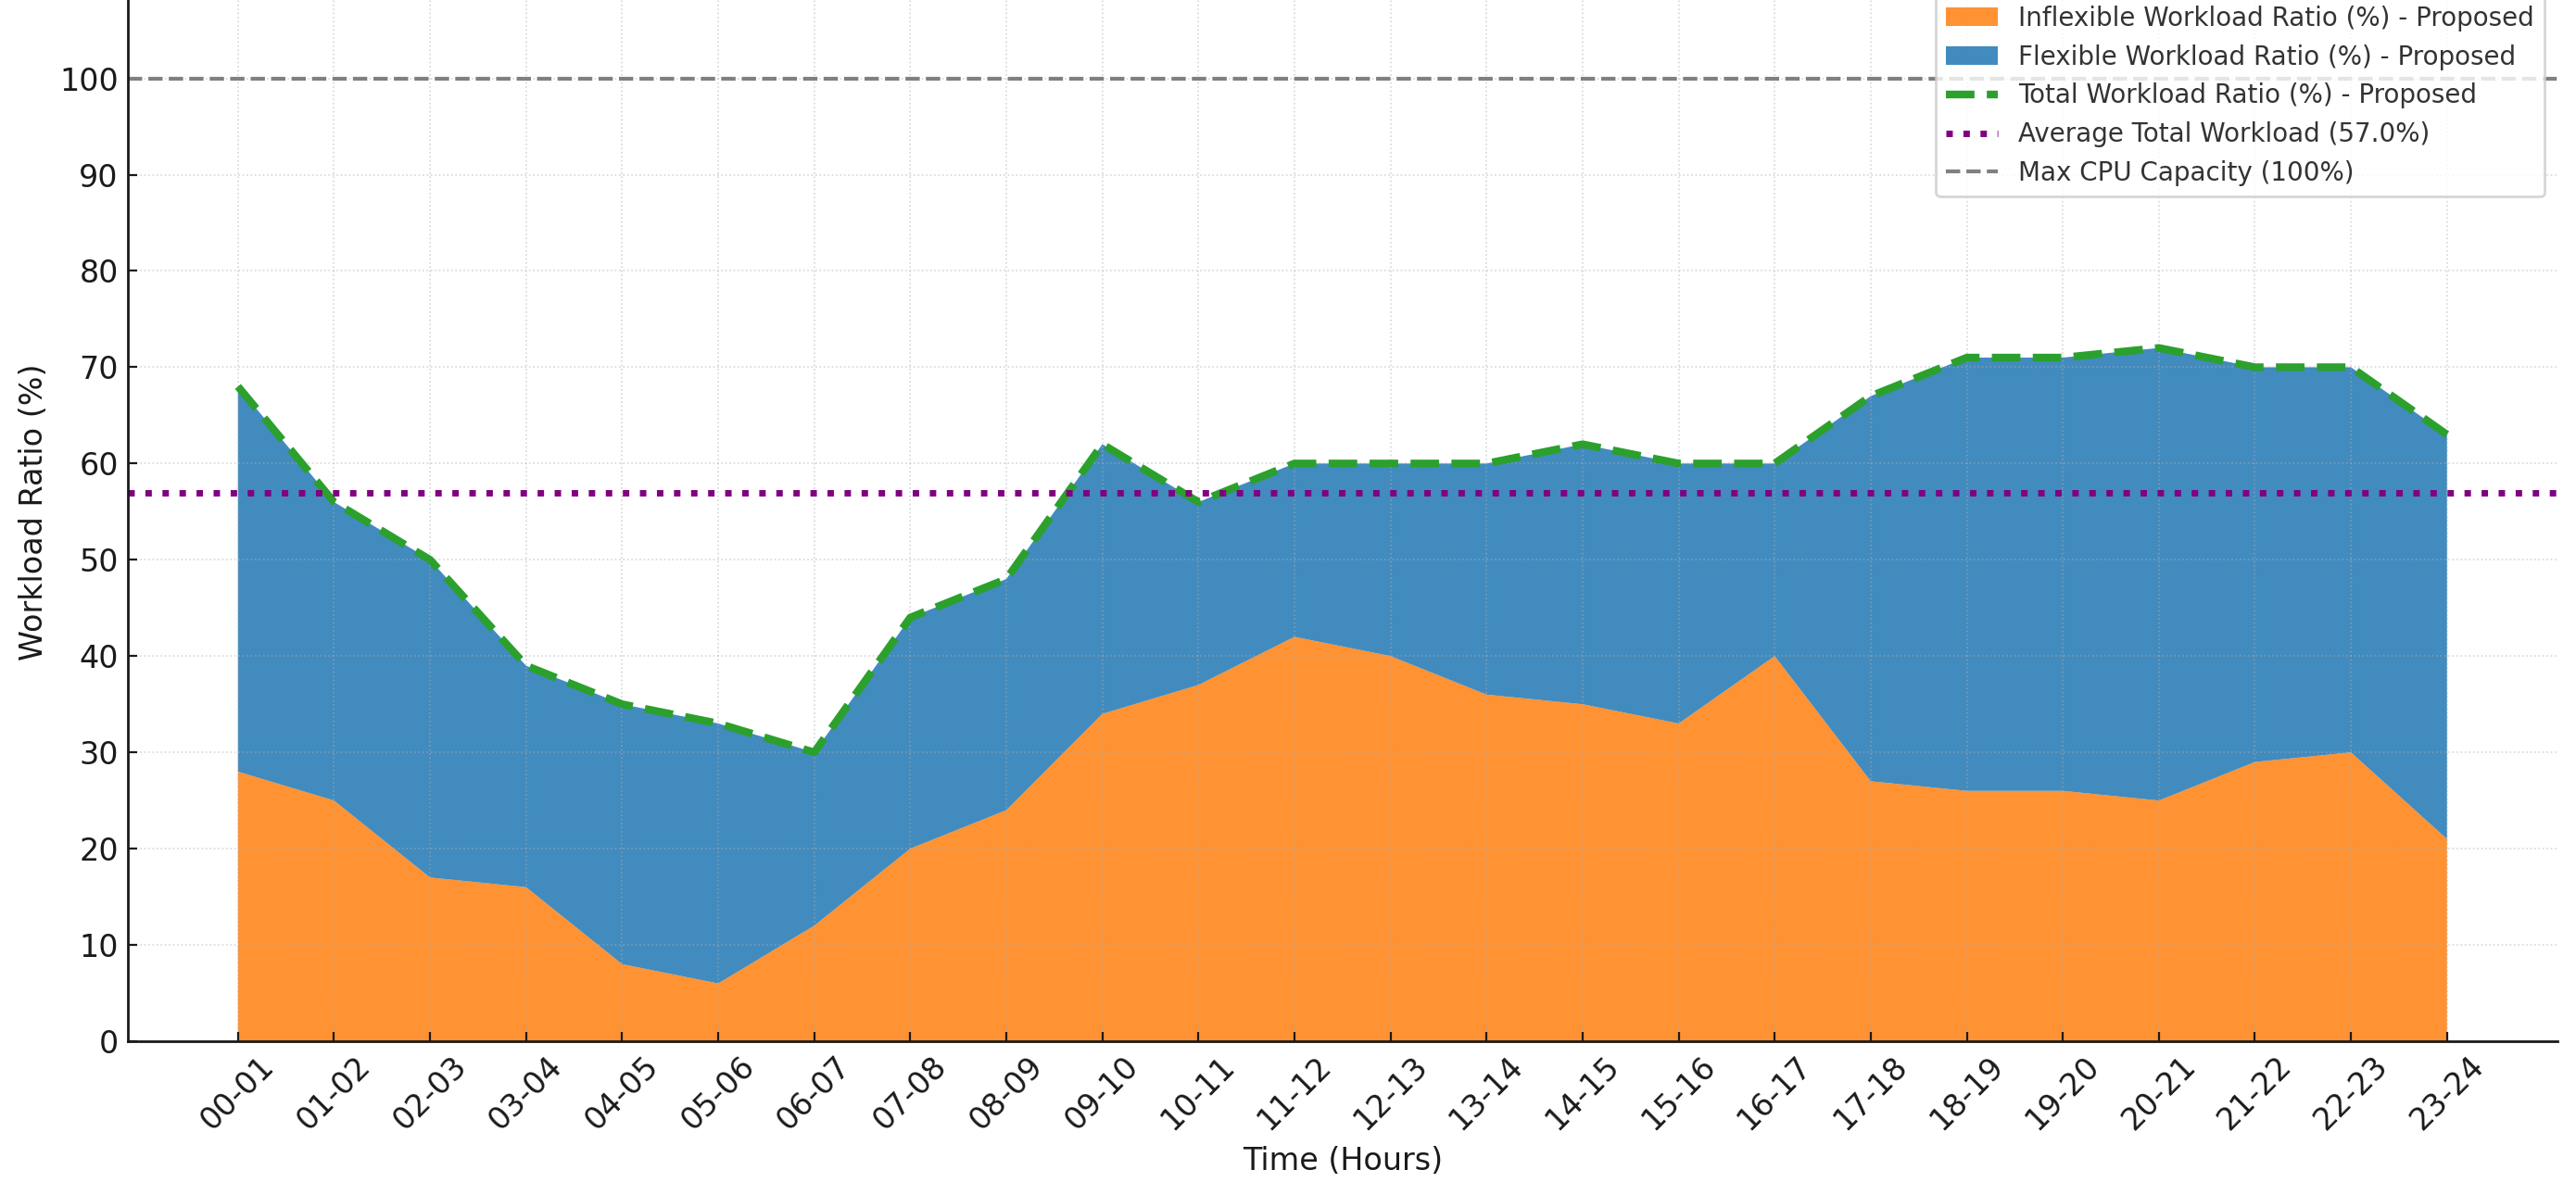
\includegraphics[width=\columnwidth]{images/Figure_2.png}
\caption{Stacked Proposed Workload Ratios Over 24 Hours}
\label{fig:workload_ratios}
\end{figure}

Categorising the deferral flexibility of IT workloads, defined as the proportion of workloads that can be shifted and the maximum duration by which they can be postponed, is essential for developing effective load-shifting strategies. Drawing on insights from various studies \cite{Centrica2020LEM, Cao2022ApEn}, a representative set of deferral windows applicable to flexible IT workloads over a 24-hour period is defined and summarised in Table~\ref{tab:shiftable}.


% --- Single-column version of your second (wide) table ---
\begin{table}[!t]
\centering
\caption{Hourly Distribution of Shiftable Workload Under Different Deferral Windows (\%)}
\label{tab:shiftable}
\setlength{\tabcolsep}{2pt} % keep your tighter column spacing
\begin{scriptsize}
\resizebox{\columnwidth}{!}{%
\begin{tabular}{ll|*{24}{c}}
\toprule
\textbf{\rev{Tranche}} & \textbf{Deferral} & \multicolumn{24}{c}{\textbf{Time}} \\
\cmidrule(l){3-26}
& & 00 & 01 & 02 & 03 & 04 & 05 & 06 & 07 & 08 & 09 & 10 & 11 & 12 & 13 & 14 & 15 & 16 & 17 & 18 & 19 & 20 & 21 & 22 & 23 \\
\midrule
\rev{$k=1$} & 0 $\leq$ 30 min & 25 & 25 & 35 & 25 & 25 & 25 & 23 & 20 & 25 & 25 & 35 & 32 & 45 & 50 & 40 & 45 & 50 & 50 & 10 & 15 & 18 & 22 & 20 & 15 \\
\rev{$k=2$} & 0 $\leq$ 60 min & 25 & 25 & 17 & 15 & 20 & 15 & 28 & 20 & 15 & 17 & 22 & 20 & 25 & 20 & 20 & 25 & 15 & 20 & 20 & 20 & 12 & 18 & 16 & 20 \\
\rev{$k=3$} & 0 $\leq$ 2 h & 20 & 15 & 18 & 20 & 15 & 15 & 15 & 15 & 13 & 16 & 13 & 15 & 15 & 15 & 25 & 15 & 20 & 15 & 30 & 25 & 25 & 25 & 24 & 20 \\
\rev{$k=4$} & 0 $\leq$ 3 h & 30 & 35 & 30 & 40 & 40 & 45 & 34 & 45 & 47 & 42 & 30 & 33 & 15 & 15 & 15 & 15 & 15 & 15 & 40 & 40 & 45 & 35 & 40 & 45 \\
\bottomrule
\end{tabular}%
}
\end{scriptsize}
\end{table}

\rev{Table~\ref{tab:shiftable} presents the hourly distribution of flexible workloads across the four delay tranches: tranche $k=1$ contains jobs that can be deferred by up to 30 minutes, $k=2$ by up to 60 minutes, $k=3$ by up to 2 hours, and $k=4$ by up to 3 hours.} The percentages represent the relative distribution within the flexible workload. For instance, during the 12:00--13:00 interval, 45\% of the flexible workloads can be deferred up to 30 minutes, 25\% for up to 60 minutes, 15\% for up to 2 hours, and the remaining 15\% for up to 3 hours. These categorized hourly workload profiles are shown in Figure \ref{fig:workload_ratios}  
and utilised as modelling inputs, capturing the time-dependent and duration-sensitive characteristics of data centre flexibility in this study.

\subsubsection{IT Power Consumption Model}

 In the literature, various approaches exist for modelling the power consumption of IT equipment, particularly servers. Given that server power consumption often constitutes the dominant portion of the total IT power draw, other components are frequently disregarded, and server power consumption is typically taken as a proxy for the overall IT power consumption. Numerous linear and non-linear models have been developed to represent server power consumption. A fundamental and widely accepted principle is that server power consumption is strongly correlated with its CPU utilisation. \rev{Based on this principle,} Equation~\ref{eq:it-power} was used in this study to estimate the electric power consumption associated with the IT workload \cite{dayarathna2015data,v2015analysis}.
\begin{equation}
P^{\mathrm{IT}}(t) = P^{\mathrm{IT}}_{\mathrm{idle}} + (P^{\mathrm{IT}}_{\mathrm{max}} - P^{\mathrm{IT}}_{\mathrm{idle}}) \times u(t)^{1.32}
\label{eq:it-power}
\end{equation}



Therefore, the flexibility provided through IT workload shifting fundamentally depends on the rescheduling of CPU utilisation over time.

The core principle of workload shifting employed in this article relies on the concept of constant computational demand for each job. This demand, denoted as $R$, is defined by the required CPU resources and the duration for which they are needed. \rev{Representing computational demand as the product of CPU utilisation and execution duration is a common approximation in aggregate workload modelling, because the total amount of computational work can be interpreted as the accumulation of processor occupancy over time \cite{dayarathna2015data,6779441,Cao2022ApEn}. For example, a workload operating at 50\% utilisation for two hours produces an equivalent computational demand to a workload operating at 100\% utilisation for one hour. This abstraction is appropriate at the facility level considered here, where the modelling target is total processor occupancy over time rather than the instruction-level execution path of individual jobs.} Execution can be at a lower or higher CPU utilisation for a longer or shorter duration respectively. In all cases, the IT job must be fully executed within the maximum delay tolerance defined by its tranche. The crucial relationship of constant computational demand for a given IT job is mathematically represented in Equation~\ref{eq:comp_demand} and conceptually illustrated in Figure~\ref{fig:constantR}.
\begin{equation}
R = u(t) \times \Delta T
\label{eq:comp_demand}
\end{equation}

\begin{figure}[!t]
 \centering
 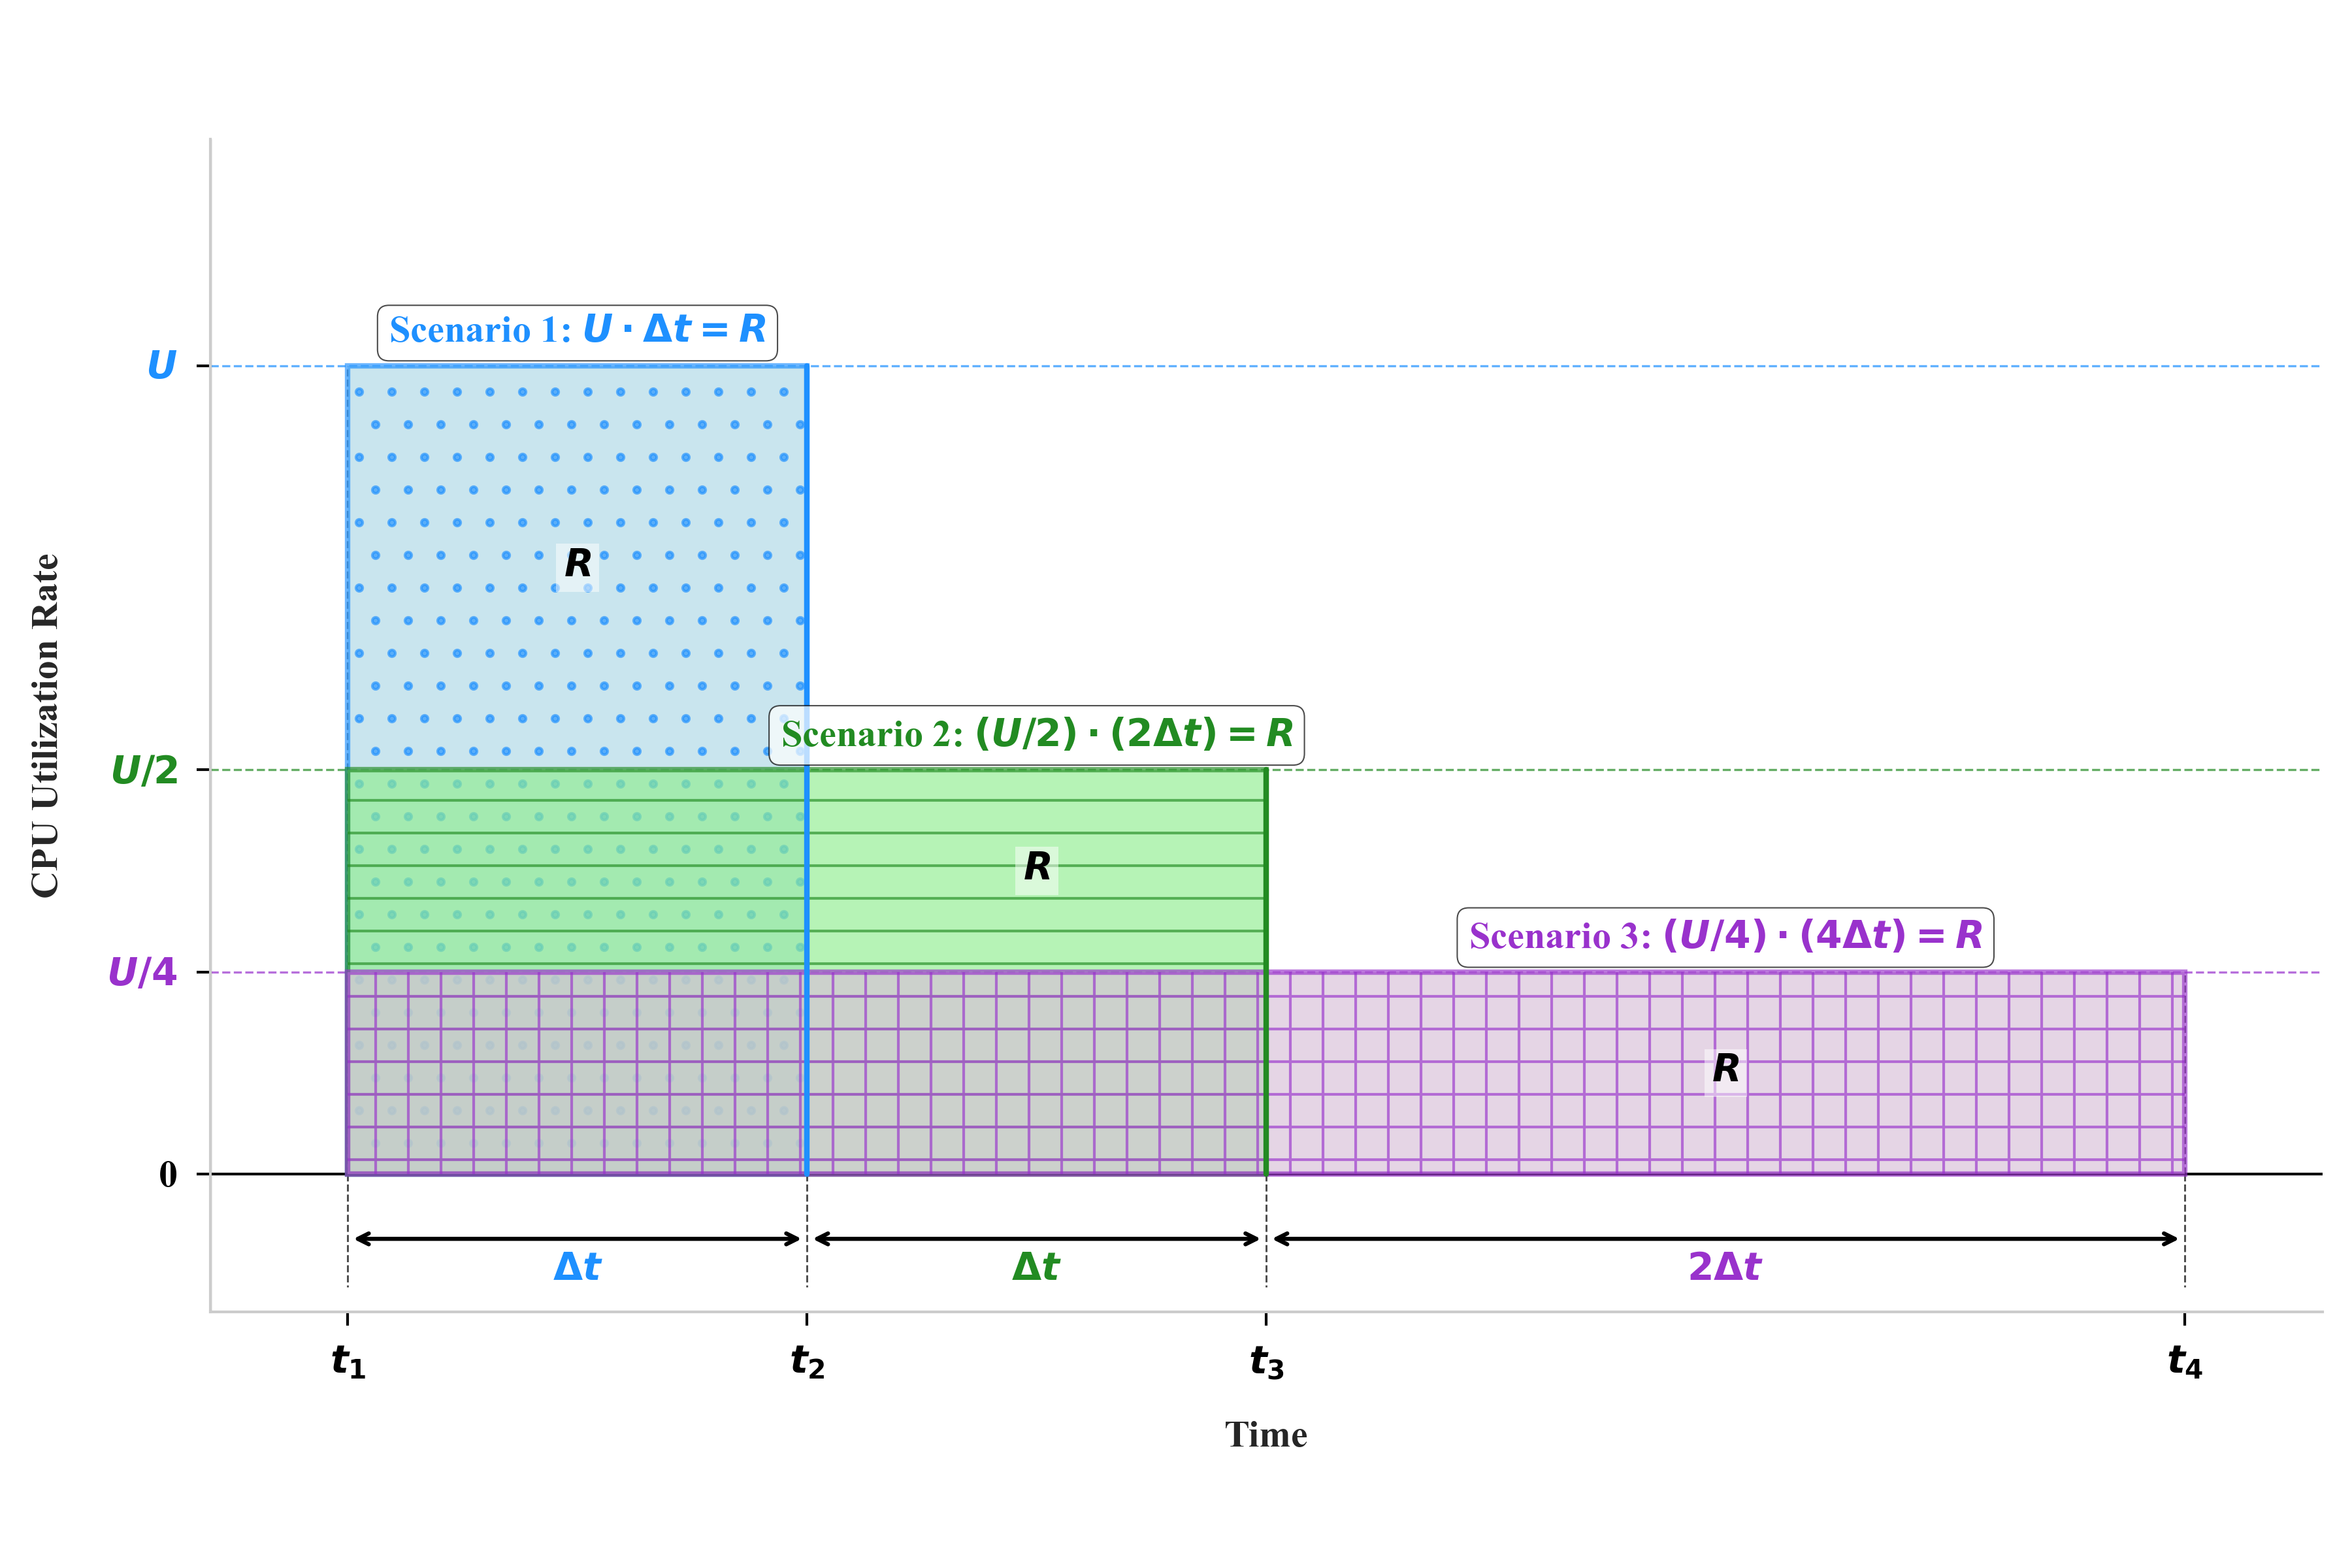
\includegraphics[width=\columnwidth]{images/Figure_3.png}
 \caption{Constant Computational Demand ($R$) with Varying CPU Utilisation and Duration}
 \label{fig:constantR}
\end{figure}


As depicted in Figure~\ref{fig:constantR}, a job with a constant computational demand $R$, can be executed over varying time frames $\Delta T$, by adjusting the allocated CPU utilisation $u(t)$. Decreasing CPU utilisation extends the job's duration, while increasing it shortens the duration, all while maintaining the same total computational demand ($R$). Consequently, the power consumption profile corresponding to the CPU utilisation changes accordingly. By strategically increasing or decreasing CPU utilisation in response to system requirements or grid signals, the associated power consumption can be modulated, enabling the provision of upward or downward flexibility, respectively.

\subsubsection{IT Workload Formulation} \label{sec:Quantifying Maximum Temporal Flexibility from IT Workload Shifting}

The annual formulation retains the four workload tranches and the time-varying
fractions reported in Table~\ref{tab:shiftable}, but represents every arrival as
a timestamped cohort. This change is necessary because work arriving near
midnight may have a deadline on the following local day. A cohort retains its
original arrival time, delay class, absolute deadline and remaining CPU-hours
when it is passed between daily optimisations.

The model conceptualises all servers in the data centre as one aggregate
computational resource. This is the same system-level simplification used in
the smaller revision: it does not model placement on individual servers, but it
does preserve the amount of computational work, its release time, deadline and
the aggregate CPU-capacity limit.

For cohort $c$, let $r_c$ be its arrival time, $d_c$ its absolute deadline and
$a_c^d$ the CPU-hours remaining when local day $d$ is opened. The feasible
execution window is $\mathcal W_c=\{t:r_c\leq t\leq d_c\}$. The decision variable
$u_{c,t}$ is the share of aggregate CPU capacity assigned to cohort $c$ in
interval $t$. The inflexible workload is executed at arrival, while flexible
cohorts may be distributed only within their corresponding window.

\begin{figure*}[!t]
\normalsize
\begin{flalign}
& \mathcal W_c=\{t:r_c\leq t\leq d_c\}
&& \label{eq:execution-window}\\[0.3\baselineskip]
& \sum_{t\in\mathcal W_c}u_{c,t}\Delta t=a_c
&& \label{eq:workload-completion}\\[0.3\baselineskip]
& u_t=u_t^{\mathrm{inflex}}+\sum_{c:t\in\mathcal W_c}u_{c,t}\leq1,
\qquad u_{c,t}\geq0
&& \label{eq:cpu-capacity}\\[0.3\baselineskip]
& a_c^{d+1}=a_c^d-\sum_{t\in\mathcal C_d\cap\mathcal W_c}
u_{c,t}\Delta t
&& \label{eq:workload-handoff}\\[0.3\baselineskip]
& u_t^{\mathrm{base}}=u_t^{\mathrm{inflex}}+
u_t^{\mathrm{flex,arrival}}
&& \label{eq:base-utilisation}\\[0.3\baselineskip]
& P_t^{\mathrm{IT,base}}=P_{\mathrm{idle}}+
(P_{\max}-P_{\mathrm{idle}})(u_t^{\mathrm{base}})^{1.32}
&& \label{eq:power-base}\\[0.3\baselineskip]
& P_t^{\mathrm{IT,opt}}=P_{\mathrm{idle}}+
(P_{\max}-P_{\mathrm{idle}})(u_t)^{1.32}
&& \label{eq:power-optimised}\\[0.3\baselineskip]
& E_t^{\mathrm{IT,base}}=P_t^{\mathrm{IT,base}}\Delta t,\qquad
E_t^{\mathrm{IT,opt}}=P_t^{\mathrm{IT,opt}}\Delta t
&& \label{eq:it-energy}
\end{flalign}
\hrulefill
\vspace*{4pt}
\end{figure*}

If $u_{c,t}$ is the utilisation assigned to the cohort at interval $t$, every
cohort whose deadline is visible in the current horizon must satisfy
Equation~\eqref{eq:workload-completion}.
Cohorts with a later deadline may remain partly unfinished, in which case their
remaining CPU hours are stored and passed to the following day. At each interval
the total scheduled utilisation is limited by Equation~\eqref{eq:cpu-capacity}.
Equations~\eqref{eq:workload-completion} and \eqref{eq:cpu-capacity} preserve the
central idea of constant computational demand: changing the execution rate can
change when a job is processed, but not the amount of work that must be
completed. This permits load shifting without treating delayed work as an
energy saving or a reduction in service quality.

The cohort representation can be understood by considering work that arrives
at noon. The part assigned to the 30 minute class may be executed at noon or in
either of the following two quarter hour intervals. Work in the three hour class
has a wider choice of execution times, but it must still be completed by 15:00.
The optimiser may spread either class over several intervals, provided that the
area under its utilisation trajectory, measured in CPU hours, equals the
original requirement. A lower execution rate requires more time, and
a higher rate completes the same work sooner. Equation~\eqref{eq:cpu-capacity}
couples all cohorts that are eligible at the same time and prevents their
combined execution from exceeding the available computing capacity.

This treatment separates temporal flexibility from demand destruction.
Deferring work can reduce grid demand in one interval, but it creates an
obligation to execute the same CPU-hours before the cohort deadline. The load
can therefore be shifted, but it cannot be discarded or postponed indefinitely.
Similarly, advancing work can increase
grid demand during a period when greater consumption is useful, but only if the
job has already arrived and computing capacity is available. These restrictions
are why the flexible share alone does not determine the response of the whole
facility. The location of deadlines, the current CPU loading and the condition
of the cooling and storage systems are all relevant.

Aggregate IT electrical power is related to CPU utilisation by
Equation~\eqref{eq:it-power}.

For a cohort that has not reached its deadline by the end of the committed core
$\mathcal C_d$, the remaining work passed to the next day is calculated using
Equation~\eqref{eq:workload-handoff}.
The arrival time and absolute deadline are not changed during this handoff.
Consequently, a cohort carried across midnight does not receive a new delay
allowance. A cohort whose deadline lies within the current optimisation horizon
is subject to Equation~\eqref{eq:workload-completion}; a later cohort may remain
partly unfinished, but Equation~\eqref{eq:workload-handoff} records exactly the
obligation that remains.

For clarity, the benchmark and optimised IT quantities can also be written in
the form used in the smaller revision, as shown in
Equations~\eqref{eq:base-utilisation}--\eqref{eq:it-energy}.
In the benchmark, flexible work is executed at arrival and storage dispatch is
disabled; it is not reclassified as a different physical workload. In the
optimised case, Equation~\eqref{eq:workload-completion} preserves the same
CPU-hours while allowing their timing to change. Unlike the earlier
extension-only expression, full facility power is modelled in both the
committed core and the look-ahead. There is therefore no subtraction of a
separate look-ahead baseline.

where $P_{\mathrm{idle}}=166.7$ kW and $P_{\max}=1000$ kW
\cite{dayarathna2015data,v2015analysis}. The nonlinear curve is represented in
the MILP by a four segment DLOG piecewise linear approximation. Nonuniform
breakpoints place more resolution at low utilisation, where the curvature is
stronger. Across $0\leq u\leq1$, the maximum approximation error is 6.241 kW,
or 0.624\% of rated IT power.

Equation~\eqref{eq:it-power} represents the aggregate servers rather than an
individual machine. The idle term captures the power drawn even when no useful
work is being executed, while the second term increases with CPU utilisation.
Because the exponent is greater than one, the incremental electrical cost of
utilisation is not constant across the operating range. Rescheduling work can
change both the timing and, to a smaller extent, the electrical energy
associated with its execution. The piecewise representation retains this shape
while allowing the annual problem to remain a mixed integer linear programme.

\subsection{UPS ESS Mathematical Model and Constraints}

The central UPS has 600 kWh of usable modelled capacity and begins the annual
run fully charged. Its minimum permitted state of charge is 50\%. Charging and
discharging efficiencies are 0.82 and 0.92. With $P^{\mathrm{UPS}}_{\mathrm{ch},t}$
and $P^{\mathrm{UPS}}_{\mathrm{dis},t}$ in kW, the complete UPS formulation is
collected below.
\begin{figure}[!t]
\centering
\normalsize
\begin{flalign}
& E^{\mathrm{UPS}}_{t+1}=E^{\mathrm{UPS}}_t+
\eta_{\mathrm{ch}}P^{\mathrm{UPS}}_{\mathrm{ch},t}\Delta t-
\frac{P^{\mathrm{UPS}}_{\mathrm{dis},t}}{\eta_{\mathrm{dis}}}\Delta t
&& \label{eq:ups-energy}\\[0.3\baselineskip]
& E^{\mathrm{UPS}}_{\min}\leq E^{\mathrm{UPS}}_t
\leq E^{\mathrm{UPS}}_{\max}
&& \label{eq:ups-bounds}\\[0.3\baselineskip]
& E_{\min}^{\mathrm{UPS}}=SoC_{\min}E_{\mathrm{base}}^{\mathrm{UPS}},
\quad E_{\max}^{\mathrm{UPS}}=SoC_{\max}E_{\mathrm{base}}^{\mathrm{UPS}}
&& \label{eq:ups-soc-limits}\\[0.3\baselineskip]
& 0\leq P^{\mathrm{UPS}}_{\mathrm{ch},t}
\leq z_t^{\mathrm{UPS}}P^{\mathrm{UPS}}_{\mathrm{ch,max}}
&& \label{eq:ups-charge-limit}\\[0.3\baselineskip]
& 0\leq P^{\mathrm{UPS}}_{\mathrm{dis},t}
\leq(1-z_t^{\mathrm{UPS}})P^{\mathrm{UPS}}_{\mathrm{dis,max}}
&& \label{eq:ups-discharge-limit}\\[0.3\baselineskip]
& P_t^{\mathrm{UPS,net}}=P_t^{\mathrm{UPS,ch}}-
P_t^{\mathrm{UPS,dis}}
&& \label{eq:ups-net}\\[0.3\baselineskip]
& P_t^{\mathrm{IT}}=P_t^{\mathrm{grid,IT}}+
P^{\mathrm{UPS}}_{\mathrm{dis},t}
&& \label{eq:ups-it-balance}
\end{flalign}
\hrulefill
\vspace*{4pt}
\end{figure}

The first power term adds the energy that reaches the battery after charging
losses. The second removes more energy from the stored state than is delivered
to the IT load, because discharge losses must also be supplied by the battery.
The equation is applied from one interval to the next, so the operating choice
made now changes the flexibility available later in the day and on subsequent
days.
The energy state is bounded by Equation~\eqref{eq:ups-bounds}; the limits are
defined explicitly by Equation~\eqref{eq:ups-soc-limits}.
For the central case, $SoC_{\min}=0.5$ and $SoC_{\max}=1$. The first annual
interval begins at $E_{\max}^{\mathrm{UPS}}$; no equation forces the battery
back to its opening energy at the end of each local day.

The lower bound preserves the minimum reserve assumed for the UPS and prevents
the optimisation from using capacity that would not be released in practice.
The upper bound prevents overcharging. Unlike the original selected day study,
the annual formulation does not require the battery to return to an artificial
daily target. Its closing energy is passed to the following day, where it remains
available or must be replenished according to the subsequent price signal.
A binary variable $z_t^{\mathrm{UPS}}$ selects the operating direction through
Equations~\eqref{eq:ups-charge-limit} and \eqref{eq:ups-discharge-limit}.
When $z_t^{\mathrm{UPS}}=1$, charging may be positive and discharge is forced to
zero. When it is zero, the reverse is true. This exclusivity is required because
simultaneous charging and discharging would waste energy and could otherwise be
used by the mathematical model to create an artificial operating point.

For reporting, its signed net power is defined by Equation~\eqref{eq:ups-net}.
Positive net power denotes charging from the grid and negative net power
denotes discharge behind the meter. This identity is retained because it makes
the component plots easy to interpret, although the optimisation itself uses
the separate non-negative charge and discharge variables.

The charging limit is 270 kW. The battery has a larger discharge nameplate, but
its useful discharge in this model cannot exceed the IT demand it supplies.
UPS discharge is placed behind the meter through
Equation~\eqref{eq:ups-it-balance}.
The UPS does not appear as an independent export from the facility.
Its discharge replaces part of the grid electricity that would otherwise supply
the IT equipment. Charging has the opposite effect and increases metered demand.
This sign convention is also important when the component results are examined:
a negative UPS contribution represents discharge behind the meter, not power
exported through a separate market connection.
This formulation is intentionally conventional. The novelty of the study does
not depend on a new battery model; it depends on how the UPS is coordinated with
workload timing and cooling, and on whether the resulting grid response can be
sustained and recovered.


\subsection{Cooling System Model}\label{sec:cooling-model}

At facility level, the cooling and TES formulation is collected below so that
the thermal balance, storage constraints, chiller conversion, node dynamics and
operating limits can be reviewed together.

\begin{figure*}[!t]
\normalsize
\begin{flalign}
& Q_t^{\mathrm{CA}}+Q_t^{\mathrm{HA}}+Q_t^{\mathrm{R}}+
Q_t^{\mathrm{ITm}}
=Q_t^{\mathrm{out}}+Q_t^{\mathrm{IT}}-Q_t^{\mathrm{cool}}
&& \label{eq:thermal-balance}\\[0.3\baselineskip]
& E^{\mathrm{TES}}_{t+1}=E^{\mathrm{TES}}_t+
\left(\eta^{\mathrm{TES}}_{\mathrm{ch}}Q^{\mathrm{TES}}_{\mathrm{ch},t}
-\frac{Q^{\mathrm{TES}}_{\mathrm{dis},t}}
{\eta^{\mathrm{TES}}_{\mathrm{dis}}}\right)\Delta t
&& \label{eq:tes-energy}\\[0.3\baselineskip]
& E^{\mathrm{TES}}_{\min}\leq E^{\mathrm{TES}}_t
\leq E^{\mathrm{TES}}_{\max}
&& \label{eq:tes-bounds}\\[0.3\baselineskip]
& 0\leq Q^{\mathrm{TES}}_{\mathrm{ch},t}
\leq z_t^{\mathrm{TES}}Q^{\mathrm{TES}}_{\mathrm{ch,max}}
&& \label{eq:tes-charge-limit}\\[0.3\baselineskip]
& 0\leq Q^{\mathrm{TES}}_{\mathrm{dis},t}
\leq(1-z_t^{\mathrm{TES}})Q^{\mathrm{TES}}_{\mathrm{dis,max}}
&& \label{eq:tes-discharge-limit}\\[0.3\baselineskip]
& Q_t^{\mathrm{cool}}=\mathrm{COP}\,P_t^{\mathrm{ch,CRAC}}+
Q^{\mathrm{TES}}_{\mathrm{dis},t}
&& \label{eq:cooling-supply}\\[0.3\baselineskip]
& Q^{\mathrm{TES}}_{\mathrm{ch},t}=\mathrm{COP}\,
P_t^{\mathrm{ch,TES}}
&& \label{eq:tes-charge-cop}\\[0.3\baselineskip]
& P_t^{\mathrm{ch,CRAC}}+P_t^{\mathrm{ch,TES}}
\leq P^{\mathrm{ch}}_{\max}
&& \label{eq:chiller-limit}\\[0.3\baselineskip]
& T_t^{\mathrm{in}}=T_{t+1}^{\mathrm{HA}}-
\frac{Q_t^{\mathrm{cool}}}{\dot m c_p}
&& \label{eq:inlet-temperature}\\[0.3\baselineskip]
& T_{t+1}^{\mathrm{IT}}=T_t^{\mathrm{IT}}+
\frac{\Delta t_s}{C_{\mathrm{IT}}}
\left[P_t^{\mathrm{IT}}-G_{\mathrm{conv}}
(T_{t+1}^{\mathrm{IT}}-T_{t+1}^{\mathrm{R}})\right]
&& \label{eq:it-temperature}\\[0.3\baselineskip]
& T_{t+1}^{\mathrm{R}}=T_t^{\mathrm{R}}+
\frac{\Delta t_s}{C_{\mathrm{R}}}
\left[\dot m\kappa c_p(T_{t+1}^{\mathrm{CA}}-T_{t+1}^{\mathrm{R}})
+G_{\mathrm{conv}}(T_{t+1}^{\mathrm{IT}}-T_{t+1}^{\mathrm{R}})\right]
&& \label{eq:rack-temperature}\\[0.3\baselineskip]
& T_{t+1}^{\mathrm{CA}}=T_t^{\mathrm{CA}}+
\frac{\Delta t_s}{C_{\mathrm{CA}}}
\left[\dot m\kappa c_p(T_t^{\mathrm{in}}-T_{t+1}^{\mathrm{CA}})
-G_{\mathrm{cold}}(T_{t+1}^{\mathrm{CA}}-T^{\mathrm{out}})\right]
&& \label{eq:cold-temperature}\\[0.3\baselineskip]
& T_{t+1}^{\mathrm{HA}}=T_t^{\mathrm{HA}}+
\frac{\Delta t_s}{C_{\mathrm{HA}}}
\left[\dot m\kappa c_p(T_{t+1}^{\mathrm{R}}-T_{t+1}^{\mathrm{HA}})\right]
&& \label{eq:hot-temperature}\\[0.3\baselineskip]
& P_t^{\mathrm{IT}}\leq Q_t^{\mathrm{cool}}
\leq(T_{t+1}^{\mathrm{HA}}-T_{\min}^{\mathrm{CA}})\dot m c_p
&& \label{eq:cooling-bounds}\\[0.3\baselineskip]
& T_{\min}^{j}\leq T_t^j\leq T_{\max}^{j},
\qquad j\in\{\mathrm{in,IT,R,CA,HA}\}
&& \label{eq:temperature-bounds}
\end{flalign}
\hrulefill
\vspace*{4pt}
\end{figure*}

In this block, each $Q$ is expressed in kW and
$Q_t^{\mathrm{IT}}=P_t^{\mathrm{IT}}$.
The implemented form of this balance is given by the individual IT-equipment,
rack, cold-aisle and hot-aisle state equations in the block. Writing the node equations
separately preserves the thermal inertia of each component instead of replacing
the facility with a single lumped temperature.


The cooling system is represented as a closed thermal circuit. The chiller can
send cooling directly to the computer room air conditioning system, or it can
produce cooling in advance and store it in the TES tank. Direct chiller output
removes heat at the time electricity is consumed. Charging the TES increases
current chiller demand but makes stored cooling available later. Discharging the
TES allows part of the cooling requirement to be met without running the chiller
at the same level. This separation between the production and use of cooling is
the source of TES flexibility.

The 1000 kWh thermal energy store has charge and discharge limits of 300 kW
thermal and efficiencies of 0.9 in both directions. Defining charging and
discharging heat flows as $Q^{\mathrm{TES}}_{\mathrm{ch},t}$ and
$Q^{\mathrm{TES}}_{\mathrm{dis},t}$, its state is given by
Equation~\eqref{eq:tes-energy} in the consolidated block.
Charging adds useful thermal energy after the charging loss has been applied,
whereas supplying $Q^{\mathrm{TES}}_{\mathrm{dis},t}$ to the CRAC removes a larger
amount from the store because of the discharge loss. As with the UPS, the TES
state is carried between local days. The optimiser cannot empty the tank at the
end of each day and assume that it is full again the following morning.
Its stored energy obeys Equation~\eqref{eq:tes-bounds}, and the paired constraints
in Equations~\eqref{eq:tes-charge-limit} and \eqref{eq:tes-discharge-limit} use a
binary mode variable to prevent simultaneous charging and discharging.
The mode constraint gives the store one physical direction in each interval.
Without it, simultaneous charging and discharging could appear in a solution
even though it provides no credible operational benefit. The energy and power
limits describe different restrictions: capacity determines how much cooling
can be moved through time, while the 300 kW ratings determine how quickly that
capacity can be charged or released.

The chiller supplies the CRAC system directly and can also charge the TES. With
a coefficient of performance $\mathrm{COP}=5$, its two conversion relations are
given by Equations~\eqref{eq:cooling-supply} and \eqref{eq:tes-charge-cop}.
In Equation~\eqref{eq:cooling-supply}, direct chiller cooling and TES discharge
combine to meet the cooling delivered to the data hall. Equation
\eqref{eq:tes-charge-cop} describes the separate chiller output sent into
storage. A COP of five means that one unit of chiller electricity produces five
units of thermal cooling under the fixed central case assumption.
The two electrical chiller loads share the 400 kW limit in
Equation~\eqref{eq:chiller-limit}.
This shared limit prevents the model from treating the CRAC and TES charging
paths as if they were supplied by two independent chillers. A decision to charge
the store can reduce the electrical capacity available for immediate
cooling, and the optimiser must retain enough capacity to keep the data hall
within its temperature limits.

The thermal model is adapted from the four node formulation of Cupelli
\emph{et al.}~\cite{cupelli2018data}. It describes the IT equipment, rack air,
cold aisle and hot aisle, while the chiller and TES determine the inlet air
temperature. The equations use consistent kW and kJ units. The inlet
temperature is defined by Equation~\eqref{eq:inlet-temperature}.
The hot aisle air is cooled before it re-enters the cold aisle. The temperature
drop is determined by the cooling supplied and by the heat capacity rate of the
circulating air, $\dot m c_p$. Increasing cooling lowers the inlet
temperature, subject to the physical limit introduced below.
The four temperature states are updated with backward Euler in
Equations~\eqref{eq:it-temperature}--\eqref{eq:hot-temperature}.
These equations describe the path followed by heat through the facility. The IT
equipment equation assumes that its electrical demand becomes heat. Part of this
heat is retained in the thermal mass of the equipment and the remainder passes
to the rack air through the conductance $G_{\mathrm{conv}}$. The rack equation
then combines that heat transfer with the flow of conditioned air from the cold
aisle. The factor $\kappa$ represents the effective fraction of the nominal air
flow participating in the exchange.

The cold aisle receives the cooled inlet air and also exchanges heat with the
outside environment through $G_{\mathrm{cold}}$. The hot aisle receives the air
leaving the racks. No corresponding external loss term is included in the hot
aisle equation because the model assumes hot aisle containment. The four heat
capacities determine how quickly the component temperatures respond. A large
thermal capacity slows the change in temperature and allows cooling electricity
to be moved for a time without immediately violating an operating bound. This is
the thermal inertia used as a flexibility resource; it is not treated as a source
of energy that can be used indefinitely.

Backward Euler is used because the air flow time constants make a 15 minute
explicit update unstable. Unlike the earlier formulation, the end states in
Equations~\eqref{eq:it-temperature}--\eqref{eq:hot-temperature} are constrained
variables rather than free initial values. The cold aisle is held between
18 and 23$^{\circ}$C, with wider physical bounds on the remaining states. The
additional condition in Equation~\eqref{eq:cooling-bounds}
prevents unvalidated accumulation of IT heat from being counted as a free
flexibility resource and avoids overcooling the inlet air.

The lower inequality requires the model to remove at least the heat rate
associated with IT operation. It was
introduced after tests showed that broad temperature bounds alone could allow
heat to accumulate in ways that had not been validated for sustained operation.
The upper inequality limits the cooling that can be delivered before the inlet
air would fall below the minimum cold aisle temperature. Together, the two
bounds ensure that cooling flexibility comes from the timing of chiller and TES
operation and from finite thermal inertia, rather than from ignoring heat or
producing physically unusable cooling.

The temperature-domain constraints applied at every interval boundary are
given by Equation~\eqref{eq:temperature-bounds}.
The cold aisle is limited to 18--23$^{\circ}$C in both the benchmark and
optimised annual cases. Wider physical ranges are applied to the remaining
thermal states as listed in the implementation appendix.

\subsection{Grid balance and objective}

Grid import includes IT demand supplied from the grid, UPS charging, both
chiller loads and a constant 53.095 kW auxiliary demand:
\begin{figure}[!t]
\centering
\small
\begin{flalign}
& P_t^{\mathrm{grid}}=P_t^{\mathrm{grid,IT}}+
P_t^{\mathrm{UPS,ch}}+P_t^{\mathrm{ch,CRAC}}+
P_t^{\mathrm{ch,TES}}+P^{\mathrm{aux}}
&& \label{eq:grid-balance}\\[0.3\baselineskip]
& 0\leq P_t^{\mathrm{grid}}\leq P_{\max}^{\mathrm{grid}}
&& \label{eq:grid-import-limit}\\[0.3\baselineskip]
& P_t^{\mathrm{grid,IT}},\;P_t^{\mathrm{UPS,ch}},\;
P_t^{\mathrm{ch,CRAC}},\;P_t^{\mathrm{ch,TES}}\geq0
&& \label{eq:grid-domain}\\[0.3\baselineskip]
& \min\sum_{t\in\mathcal H_d}
\pi_tP_t^{\mathrm{grid}}\Delta t/1000
&& \label{eq:objective}
\end{flalign}
\hrulefill
\vspace*{4pt}
\end{figure}
Equation~\eqref{eq:grid-balance} is written at the facility meter. UPS discharge
does not appear as a separate negative term because its effect has already been
accounted for in $P_t^{\mathrm{grid,IT}}$ through Equation
\eqref{eq:ups-it-balance}. In contrast, UPS charging is an additional metered
load. TES discharge also enters indirectly by reducing the direct chiller power
needed to satisfy Equation~\eqref{eq:cooling-supply}. This accounting prevents
the same storage action from being counted twice.

The model represents import only. Its electrical variables satisfy
the import limit in Equation~\eqref{eq:grid-import-limit} and the non-negativity
domain in Equation~\eqref{eq:grid-domain}.
The structural central-case limit is 1723.095 kW. This prevents the UPS from
being interpreted as a separate exporting generator and makes the sign
convention at the facility meter explicit.

For each daily solve, the objective is given by Equation~\eqref{eq:objective},
where $\mathcal H_d$ contains the committed day and its look ahead and $\pi_t$
is the signed IMRP in GBP/MWh. Calendar year reporting includes only committed
2025 intervals, so the overlapping look ahead is never counted twice. Storage
degradation, standing losses, network charges and terminal energy credits are
not included in the central objective.

Because $\pi_t$ is signed, moving consumption from a high positive price interval
to a low or negative price interval can reduce cost even when total electricity
use rises. The objective represents participation in an energy market,
not a complete retail electricity bill. A demand charge, connection constraint
or degradation cost would change the relative value of high charging power and
could discourage some of the peaks observed in the optimised result.


\subsection{365-Day Rolling-Horizon Formulation}\label{sec:annual-rolling}

The model represents an aggregate data centre with 1 MW of rated IT power. The
purpose of the model is not to reproduce the placement of individual jobs or
the airflow around individual racks. It is to retain the states that determine
whether the facility can alter its grid demand without losing computational
work or moving the thermal and storage consequences outside the study window.
Those states are the unfinished flexible workload, UPS and TES energy, the
temperatures of the IT equipment, rack, cold aisle and hot aisle, and total grid
import. This level of detail preserves the main interactions between computing,
electrical storage and cooling while allowing the optimisation to be solved
repeatedly over a complete year.

Time is divided into 15 minute intervals. Each solve contains one local calendar
day followed by a 12 interval look ahead. A normal day therefore has 96
committed intervals, while the spring and autumn daylight saving transitions
have 92 and 100. The additional three hours expose the latest deadline of every
job that arrives during the committed day. Only the committed intervals enter
the reported annual cost; the look ahead is used to protect workload completion
and provide a feasible continuation.

At the end of local day $d$, the physical state
\begin{equation}
 \boldsymbol{x}_{d}^{\mathrm{end}}=
 (E^{\mathrm{UPS}},E^{\mathrm{TES}},T^{\mathrm{IT}},T^{\mathrm{R}},
 T^{\mathrm{CA}},T^{\mathrm{HA}})
 \label{eq:state-vector}
\end{equation}
is imposed as the opening state of day $d+1$. Unfinished workload is passed
forward separately as a set of cohorts. Each cohort retains its original arrival
time, its absolute deadline and its remaining CPU hours. This is important:
resetting either the physical states or the workload at midnight would create
energy or computing capacity that the data centre does not actually possess.

\begin{figure*}[!t]
\centering
\resizebox{\textwidth}{!}{%
\begin{tikzpicture}[
 node distance=7mm and 9mm,
 block/.style={draw,rounded corners,align=center,minimum height=9mm,
 minimum width=26mm,fill=blue!6,font=\small},
 decision/.style={draw,diamond,aspect=2,align=center,fill=orange!10,font=\small},
 arrow/.style={-{Latex[length=2mm]},thick}]
 \node[block] (inputs) {Build signed price and\\workload timeline};
 \node[block,right=of inputs] (open) {Load physical state and\\deadline cohorts};
 \node[block,right=of open] (solve) {Solve daily core plus\\three hour look ahead};
 \node[block,right=of solve] (audit) {Audit feasibility, cost,\\states and workload};
 \node[decision,right=of audit] (last) {Final local\\day?};
 \node[block,below=of solve] (commit) {Commit core; store end state,\\cohorts and dispatch};
 \node[block,below=of last] (annual) {Reconcile annual totals and\\run endpoint analyses};
 \draw[arrow] (inputs)--(open);
 \draw[arrow] (open)--(solve);
 \draw[arrow] (solve)--(audit);
 \draw[arrow] (audit)--(last);
 \draw[arrow] (last)--node[right,font=\scriptsize]{no}(commit);
 \draw[arrow] (commit.west)-| (open.south);
 \draw[arrow] (last)--node[right,font=\scriptsize]{yes}(annual);
\end{tikzpicture}
}
\caption{Linked annual optimisation workflow. The stored checkpoint from one
local day supplies the opening state of the next day and, later, the opening
state of the representative day flexibility study.}
\label{fig:annual-workflow}
\end{figure*}

Figure~\ref{fig:annual-workflow} shows the complete workflow. Each committed day
is accompanied by a checkpoint and an audit record, so an interrupted annual run
can resume from the last verified state. An absolute UTC timeline prevents
missing or duplicated intervals, while local dates define the settlement day.
